\documentclass[pre, superscriptaddress, twocolumn,pre]{revtex4-1}
\usepackage{amsmath, amssymb, color, graphicx}
\definecolor{linkcolor}{rgb}{0,0,0.6} 
\usepackage[pdftex,colorlinks=true,
	pdfstartview = FitV,
	linkcolor    = linkcolor,
	citecolor    = linkcolor,
	urlcolor     = linkcolor,	
	hyperindex   = true,
	hyperfigures = false]{hyperref}

\newcommand{\dd}{\text{d}}
\newcommand{\ee}{\text{e}}
\newcommand{\ii}{\text{i}}


% ===============================================================================


\begin{document}

\title{How does dissipation constrain fluctuations beyond equilibrium?\\Renormalization of transport and structure in a driven liquid due to energy flows}

\author{Laura Tociu}
\affiliation{James Franck Institute, University of Chicago, Chicago, IL 60637}
\affiliation{Department of Chemistry, University of Chicago, Chicago, IL 60637}

\author{\'Etienne Fodor}
\affiliation{DAMTP, Centre for Mathematical Sciences, University of Cambridge, Wilberforce Road, Cambridge CB3 0WA, UK}

\author{Takahiro Nemoto}
\affiliation{Philippe Meyer Institute for Theoretical Physics, Physics Department, \'Ecole Normale Sup\'erieure \& PSL Research University, 24, rue Lhomond, 75231 Paris Cedex 05, France}

\author{Suriyanarayanan Vaikuntanathan}
\affiliation{James Franck Institute, University of Chicago, Chicago, IL 60637}
\affiliation{Department of Chemistry, University of Chicago, Chicago, IL 60637}

\begin{abstract}
	In this paper we study the implications of energy flow or work done by external drives on the transport and structural properties of a liquid. First, using a theoretical model of a driven liquid, we put forward a relation between the spontaneous fluctuations, quantified by the diffusion coefficient, and the amount of work produced by an external drive, related to energy dissipation. Next, we demonstrate how the hierarchy between density correlations, which enforces the fluid structure, is now affected by sustained energy dissipation. Finally, by harvesting trajectories that preferentially dissipate or absorb energy, we predict how energy flows can renormalize the interactions between particles of the liquid. These predictions are confirmed with atomistic simulations. Together, our results show how the various emergent collective excitations in many body interacting systems can be accurately controlled or tuned at the cost of energy dissipation. 
	\end{abstract}

\maketitle 


% ===============================================================================


\section{Introduction}

Non-equilibrium forces can drive novel and specific pathways to modulate self-assembly and organization in materials. The close connection between energy dissipation and organization is especially apparent in living systems~\cite{Toyabe2010, Ahmed2016, Battle604}. As an example, the flagella motors of {\it E. Coli} exhibit a unique phenomenology combining ultra-sensitive response, adaptation, and motor restructuring as a function of the applied torque~\cite{Lele2013, Lan2012, Wang2017}. Moreover, both {\it in vivo} studies of the cellular cytoskeleton, as well as {\it in vitro} experiments on model systems of actin and/or microtubule networks driven by molecular motors, have also shown that non-equilibrium forces control a large variety of functionality in the cell~\cite{Silva2011, Sanchez2012, Blanchoin2014, Murrell2015}. They have demonstrated, for instance, how living systems can robustly sense forces, and therefore constantly adapt to their surroundings~\cite{Decamp2015}. 


To elucidate the role of non-equilibrium forces in material properties, it is crucial to first examine how sustained energy flows affect the dynamics. While the features of equilibrium settings are well established, progress in controlling non-equilibrium systems has been hampered by a lack of general principles~\cite{Takatori2015, Cates2015, Solon2015a, Nguyen2016, Fodor2016, Murugan2017, Nguyen2018}. For instance, the canonical relation between fluctuation and dissipation no longer holds, its violation is directly related to the work applied by non-equilibrium forces~\cite{Harada2005, Harada2006}. Understanding the interplay between the energy dissipated by these non-equilibrium forces and resulting structure and organization is an open and important problem~\cite{Mizuno2007, Wilhelm2008, Visco2015, Turlier2016, Nardini2017}.


In a recent work, some of the present authors have reported empirical relations between dissipation, transport and emerging phases in a model driven system~\cite{Han2016, delJunco2018}. The scaling behaviors are captured by a phenomenological model for density fluctuations, without any explicit connection with the underlying dynamics~\cite{Chandler1993}. It remains to be seen if simple scaling results can be obtained within settings where coarse-graining and interactions between particles is treated more rigorously~\cite{Dean1996, Demery2011, Demery2014}. Moreover, it has been shown recently that changing dissipation, by biasing trajectories externally~\cite{Lecomte2007, Touchette2009, Jack2010}, strongly affects the density correlations of non-equilibrium fluids~\cite{Nemoto2018a}. This motivates the search for some generic predictions on how controlling dissipation rates can constrain the emerging structures.


In this paper, we explore how energy flows modify the properties of a class of driven liquids. We first consider a driven tracer in a generic Gaussian fluctuating field~\cite{Chandler1993, Dean1996, Demery2014, Kruger2017}. The Gaussian field  is meant to mimic a liquid of interacting particles~\cite{Chandler1993}. We derive expressions for the diffusion coefficient of driven particles and the work performed by the drive by treating the interactions between the tracer and Gaussian field perturbatively. Specifically, in the limits of large and small drive period, we find that the work and diffusion exhibit the same scaling in terms of drive amplitude and period, illustrating the interplay between dissipation and transport in this non-equilibrium system. We compare our predictions with numerical simulations of Brownian particles. A periodic external drive is applied to only a small fraction of particles, with an orbit determined by both the drive amplitude and its time period. While the interactions between the particles in the simulations are strong, the scaling of the diffusion constant and work performed with the amplitude of the driving force matches predictions from the theoretical treatment. Next, we obtain a generic relation between work and force fluctuations, from which we explore how density correlations in the driven liquid are modified due to the non-equilibrium driving. These results demonstrate how energy consumption can modify the structure and transport properties of the liquid. 

Finally, in the last section of the paper, we consider ensembles where trajectories are biased with energy flows, using methods of large deviations~\cite{Chetrite2013, Jack2010}. At first order, we reveal that the auxiliary dynamics associated with these biased ensembles simply amounts to renormalize the strength of interactions. Direct sampling of biased trajectories \textcolor{blue}{using cloning algorithm \cite{Giadina2006,tailleur2007probing,Hurtado2009,Nemoto2016,Ray2018,Klymko2018,Brewer2018}} confirm that tuning energy fluxes leads to changing the fluid structure in a controlled manner. Together, these results show how energy dissipation can modify the structure and transport properties of a fluid in a controlled manner. 


% ===============================================================================


\section{Methods}\label{sec:method}

\subsection{Theoretical model}

Our goal is to formulate a minimal model which reproduces the statistics of a tracer evolving in a liquid with Gaussian density fluctuations~\cite{Chandler1993}. To this aim, we consider the Hamiltonian of a Gaussian density field interacting with a tracer with position ${\bf r}_0$:
\begin{equation}
	\begin{aligned}
		H &= \frac{T}{2} \int \delta \rho ({\bf r}) \chi^{-1}({\bf r} - {\bf r}') \delta \rho ({\bf r}') \dd{\bf r}\dd{\bf r}'
		\\
		&\quad + \int V({\bf r}-{\bf r}_0) \delta \rho({\bf r}) \dd{\bf r} ,
	\end{aligned}
\end{equation}
where $T$ is the bath temperature, and we have set the Boltzmann constant to unity $k_\text{\tiny B}=1$. The density fluctuations around the average density $\rho_0$ are defined as $\delta \rho({\bf r},t ) = \rho({\bf r}, t) - \rho_0 $. The density covariance $\chi$ is written in terms of the two point correlation function $g$ as $\chi({\bf r}-{\bf r}')= \langle \delta \rho({\bf r}) \delta \rho ({\bf r}') \rangle=  \rho_0 \delta({\bf r} - {\bf r}') +\rho_0^2 g({\bf r}-{\bf r}')$. The equation of motion of the density field can then be written as
\begin{equation}\label{eq:EvolutionField}
	\begin{aligned}
		\frac{\partial \delta \rho({\bf r}, t)}{\partial t} &= D_\text{\tiny G} \nabla^2 \int \chi^{-1} ({\bf r}-{\bf r}') \delta \rho({\bf r}', t) \dd{\bf r}'
		\\
		&\quad + \frac{1}{\gamma_\text{\tiny G}} \nabla^2 V({\bf r}-{\bf r}_0(t)) + \nabla \cdot {\boldsymbol\Lambda}({\bf r},t) ,
	\end{aligned}
\end{equation}
where $D_\text{\tiny G} = T/\gamma_\text{\tiny G}$, and $\gamma_\text{\tiny G}$ is the field damping coefficient. The term $\boldsymbol\Lambda$ is a zero-mean Gaussian white noise with correlations
\begin{equation}
	\langle \Lambda_\alpha({\bf r}, t) \Lambda_\beta({\bf r}', t') \rangle = 2 D_\text{\tiny G} \delta_{\alpha\beta}\delta({\bf r} - {\bf r}')\delta(t-t') .
\end{equation}
In Fourier space, Eq.~\eqref{eq:EvolutionField} becomes
\begin{equation}\label{eq:FourierEvolutionField}
	\begin{aligned}
		\frac{\partial \delta \rho({\bf q},t)}{\partial t} &= - |{\bf q}|^2 \left[ D_\text{\tiny G} \chi^{-1}({\bf q}) \delta \rho({\bf q},t) + \frac{V({\bf q})}{\gamma_\text{\tiny G}} \ee^{-\ii {\bf q} \cdot {\bf r}_0(t)} \right]
		\\
		&\quad + \ii{\bf q}\cdot{\boldsymbol\Lambda} ({\bf q},t) .
	\end{aligned}
\end{equation}
The complementary equation of motion for the tracer reads
\begin{equation}\label{eq:EvolutionTracer}
	\dot{\bf r}_0 = \frac{1}{\gamma} \left( {\bf F}_\text{c}+{\bf F}_\text{d} \right) + {\boldsymbol\eta_0} ,
\end{equation}
where $\gamma$ is the tracer friction coefficient. The conservative force ${\bf F}_\text{c}$ embodies the interaction with the field $\delta\rho$:
\begin{equation}
	{\bf F}_\text{c}(t) = - \int \ii{\bf q} V(-{\bf q})\ee^{\ii{\bf q} \cdot {\bf r}_0(t)} \delta \rho({\bf q}, t) \frac{\dd{\bf q}}{(2\pi)^d} ,
\end{equation}
where $d$ refers to the spatial dimension. The term ${\boldsymbol\eta}_0$ is a zero-mean white Gaussian noise with correlations
\begin{equation}
	\langle\eta_{0\alpha}(t)\eta_{0\beta}(0)\rangle = 2 D_0 \delta_{\alpha\beta}\delta(t) ,
\end{equation}
where $D_0 = T/\gamma$. The tracer is driven out of equilibrium by the driving force ${\bf F}_\text{d}$, taken in two dimensions as
\begin{equation}\label{eq:theta}
	{\bf F}_{\rm d}(t) = A \left[\sin(2\pi t/\tau) \hat{\bf e}_x + \cos(2\pi t/\tau)\hat{\bf e}_y \right] ,
\end{equation}
where $A$ and $\tau/2\pi$ are respectively the amplitude and the period of the drive. The relative strength of the drive can be expressed in terms of the P\'eclet number $\text{Pe}$, defined as $\text{Pe} = \sigma A/\gamma D_0$, where $\sigma$ is the typical tracer size~\cite{Han2016, delJunco2018}. In the following, we define a unit vector ${\bf v}(t) \equiv {\bf F}_{\rm d}(t)/A$ to keep track of the orientation of the driving force. In the absence of interactions with the field $\delta\rho$, the average tracer position follows a periodic orbit, correspondig to a circle in two dimensions. The field dynamics~\eqref{eq:FourierEvolutionField} can be exactly solved. Specifically, by labeling $\chi^{-1}({\bf q}) = K({\bf q})$, we get
\begin{equation}
	\begin{aligned}
		\delta\rho({\bf q},t) &= \int_{-\infty}^t \dd s \ee^{-D_\text{\tiny G} |{\bf q}|^2 K({\bf q})(t-s)}
		\\
		&\quad\times \left[ \ii{\bf q} \cdot {\boldsymbol\Lambda}({\bf q},s) - |{\bf q}|^2 \frac{V({\bf q})}{\gamma_\text{\tiny G}} \ee^{-\ii {\bf q}\cdot {\bf r}_0(s)}\right] ,
	\end{aligned}
\end{equation}
yielding
\begin{equation}\label{eq:ConservativeForce}
	\begin{aligned}
		{\bf F}_\text{c}(t) &= \int \frac{\dd{\bf q}}{(2\pi)^d} \ii{\bf q} V(-{\bf q}) \ee^{\ii{\bf q} \cdot {\bf r}_0(t)} \int_{-\infty}^t \dd s \ee^{-D_\text{\tiny G} |{\bf q}|^2 K({\bf q})(t-s)}
w		\\
		&\quad\times \left[ |{\bf q}|^2 \frac{ V({\bf q})}{\gamma_\text{\tiny G}} \ee^{-\ii{\bf q} \cdot {\bf r}_0(s)} - \ii{\bf q} \cdot {\bf\Lambda}({\bf q}, s) \right] .
	\end{aligned}
\end{equation}
Following stochastic thermodynamics~\cite{Sekimoto1998, Seifert2012}, the average rate at which energy is dissipated into the thermostat $\cal J$ is simply defined as the power of the forces exerted by the driven tracer on the solvent: ${\cal J} = \gamma \langle\dot{\bf r}_0\cdot(\dot{\bf r}_0-{\boldsymbol\eta}_0)\rangle$. It can be separated into free motion and interaction contributions as ${\cal J} = \langle{\bf F}_\text{d}^2\rangle/\gamma - \dot w$, where
\begin{equation}\label{eq:work}
	\dot{w} = -\frac{1}{\gamma} \langle{\bf F}_\text{c}\cdot {\bf F}_\text{d}\rangle .
\end{equation}
Then, the rate of work $\dot w$ is the main quantity of interest to investigate how dissipation relates with properties of the system.

In this work, we have simply proposed the dynamics in Eq.~\ref{eq:EvolutionField} starting from a Gaussian field theory for density fluctuations. 
Using a systematic coarse-graining procedure~\cite{Dean1996}, the dynamics for the density field of the undriven particles can in fact be derived in terms of pair-wise potential $V$. The linearization around the average value $\rho_0$ leads to~\eqref{eq:FourierEvolutionField}, where $D_\text{\tiny G}=\rho_0D_0$, $1/\gamma_\text{\tiny G}=\rho_0$ and $\chi^{-1}({\bf q}) = 1/\rho_0 + V({\bf q})/D_0$~\cite{Demery2011, Demery2014}. In practice, such a density dynamics should only be valid for weak interactions {\it a priori}, yet previous works have shown that it remains qualitatively relevant even beyond this regime~\cite{Demery2015, Martin2018}. Indeed, Gaussian field theories for density fluctuations provide a very good description of the thermodynamics of liquids~\cite{Chandler1993}.


% -------------------------------------------------------------------------------


\subsection{Simulation details}

We simulate a set of repulsive particles in two dimensions, evolving in a box  of size $10^2\sigma\times 10^2\sigma$ at average density $\rho_0=0.45$ with periodic boundary conditions. The particles obey the following Brownian dynamics
\begin{equation}\label{eq:xEOM}
	\dot{\bf r}_i = \frac{1}{\gamma} \left({\bf F}_{{\rm c},i} + {\bf F}_{{\rm d},i}\right) + {\boldsymbol\eta}_i .
\end{equation}
The term ${\boldsymbol\eta}_i$ is a zero-mean white Gaussian noise with correlations
\begin{equation}
	\langle \eta_{i\alpha}(t)\eta_{j\beta}(0)\rangle = 2D_0\delta_{ij}\delta_{\alpha\beta}\delta(t) .
\end{equation}
The conservative force ${\bf F}_{{\rm c},i}$ applied on particle $i$ derives from a pair-wise potential, taken as a Weeks-Chandler-Andersen (WCA) potential~\cite{WCA1971}. The driving force ${\bf F}_{{\rm d},i}$ only acts on ten percent of the particles, with independent dynamics for each one of them given by Eq.~\eqref{eq:theta}. 


We run simulations using the LAMMPS simulation package with added fixes. We use some in-house analysis scripts to extract our results. All the time scales are expressed in units of the diffusive time scale $\sigma^2/D_0$, where the WCA cut-off parameter $\sigma$, analogous to the typical particle size, is set to unity. The time step is $5.10^{-4}$. The system is first relaxed for $10^5$ time steps, and later equilibrated for $50\tau$. We ran simulations at $\tau$ values of $\{20,30,40,50\}$, and $\text{Pe}$ values of $\{6,12,18,24,30,36\}$. The main quantities of interest are the rate of work $\dot w$ and the diffusion coefficient of driven particles. We evaluate average values over trajectories of length $300\tau$. We are also interested in the pair correlation function of density $g$, extracted from an average over trajectories of length $150 \tau$. 


\begin{figure}
	\centering
	\includegraphics[width=.95\linewidth]{D_active_vs_Pe_10p4.pdf}
	\includegraphics[width=.95\linewidth]{dwvsPe.pdf}
	\caption{\label{fig:diffusion}
		(Top) Diffusion coefficient $D$ of driven particles as a function of $\rm Pe$, for $\tau= 20$ (green), $30$ (yellow) and $40$ (blue). Here, $\text{Pe}$ is the P\'eclet number and is defined as $\text{Pe} = \sigma A/\gamma D_0$, where $\sigma$ is the typical tracer size, $A$ is the amplitude of driving forces and $\gamma$ is the damping constant. The lines are fits to the functional form $D = D_{\rm eq} + a(\tau) {\rm Pe} + b(\tau) {\rm Pe}^2$ with $a(20)/b(20)\approx -0.04$, $a(30)/b(30)\approx -0.09$, $a(40)/b(40)\approx 0.25$. (Bottom) $\langle \dot{w} \rangle$ as a function of $Pe$ for the same range of values of $\tau$. The lines are fits of $\langle \dot{w} \rangle$ to quadratic functions of $Pe$, $\langle \dot{w}\rangle \propto Pe^2$. 
	}
\end{figure}
% ===============================================================================


\section{Connecting energy dissipation and diffusion}\label{sec:diff}

Our first aim is to derive explicit expressions for the tracer diffusion coefficient $D$, defned as $D = \underset{t\to\infty}{\lim} (1/2dt) \big\langle \big[\langle{\bf r}_0(t)\rangle-{\bf r}_0(t)\big]^2 \big\rangle$, and the rate of dissipated work $\dot w$ given in~\eqref{eq:work}. The tracer dynamics, given in its closed form by Eqs.~\eqref{eq:EvolutionTracer} and~\eqref{eq:ConservativeForce}, can be used to set up a perturbation in terms of the interactions between the tracer and the density field $\delta\rho$. Specifically, following Refs~\cite{Demery2011, Demery2014}, we scale the potential $V$ by a small parameter $h$ in Eq.~\eqref{eq:ConservativeForce}, so that the tracer is uncoupled from the bath when $h=0$. We also present all our results in terms of $K({\bf q}) \equiv \chi^{-1}({\bf q})$ where $\chi({\bf q})$ is the Fourier transform of the two point density-density correlation function $\chi({\bf r}-{\bf r}')= \langle \delta \rho({\bf r}) \delta \rho ({\bf r}')\rangle$ defined in Section~\ref{sec:method}. 


The perturbation theory detailed in~\cite{Supplemental} allows us to extract how the rate of work performed on the system, $\dot w$, and the diffusion constant $D$ scale in various limits. In the limit of high frequencies $\omega/K({\bf q})\gg 1$, and small orbit sizes ${\rm Pe}/\omega \ll 1$, we find that the rate of work performed on the tracer particle scales like
\begin{equation}\label{eq:workscalingsmall}
	\dot w  = \left[\frac{h{\rm Pe}}{\omega\gamma}\right]^2 \frac{1}{2D_0}\int \frac{ {|{\bf q}|}^2 |V({\bf q})|^2}{K({\bf q})} \frac{\dd{\bf q}}{(2\pi)^d} .
\end{equation}
At the same time we find that the increase in the diffusion constant of the tracer particle $D-D_{\rm eq}$ scales like 
\begin{equation}\label{eq:Dscaling}
	D-D_{\rm eq} = \left[\frac{h{\rm Pe}}{\omega\gamma}\right]^2 \int \dfrac{|{\bf q}|^2 |V({\bf q})|^2 } { K({\bf q}) \left[ D_\text{\tiny G}  K({\bf q}) +  D_0 \right]} \frac{\dd{\bf q}}{(2\pi)^d} \,,
\end{equation}
where $D_{\rm eq}$ is the diffusion constant of the tracer particle under equilibrium conditions. 
These results are valid to quadratic order in $h$, the parameter that sets the strength of coupling between the tracer and the bath. They show that the renormalization of the diffusion constant can be simply written down in terms of the rate at which work is performed on the system by the non-equilibrium forces. 


In the opposite limit of low frequencies $\omega/K({\bf q}) \ll 1$, we get
\begin{equation}\label{eq:avgForceFullperturb}
	\begin{aligned}
		\dot w &= \left[\frac{h{\rm Pe}}{\gamma}\right]^2 \frac{1}{D_0} \int \frac{\dd{\bf q}}{(2\pi)^d} \frac{|V({\bf q})|^2}{K({\bf q})}
		\\
		&\quad \times \frac{D_\text{\tiny G} K({\bf q}) + D_0}{\left[D_\text{\tiny G} K({\bf q}) + D_0 \right]^2 + ({\bf q} \cdot {\rm Pe}{\bf v}/\gamma)^2 / |{\bf q}|^4} .
	\end{aligned}
\end{equation}
In the limit where the tracer particles are driven in long slow orbits ${\rm Pe}\ll K({\bf q})$, the rate of work $\dot w$ in Eq.~\eqref{eq:avgForceFullperturb} scales with ${\rm Pe}^2$. In the same limits, the expression for the diffusion constant is 
\begin{equation}
	D - D_{\rm eq} = 5 \left[\frac{h{\rm Pe}}{\gamma^2}\right]^2 \int \frac{ |V({\bf q})|^2 } { K({\bf q}) \left[ D_\text{\tiny G}  K({\bf q}) +  D_0 \right]^2} \frac{\dd{\bf q}}{(2\pi)^d} .
\end{equation}
Again, our perturbation theory shows that the renormalization of the diffusion constant of the tracer particle can simply be written in terms of the average rate at which work is done on the tracer particle. 


We extract the diffusion coefficient $D$ and the rate of work $\dot w$, from direct simulations of the microscopic dynamics~\eqref{eq:xEOM}, as described in Sec.~\ref{sec:method}. These simulations are not in the weak coupling regime $h \ll 1 $, and as such, the results of the perturbation theory described above are not applicable {\it quantitatively}. Nonetheless, this perturbation can help elucidate the scaling observed in the simulations. Specifically, our results show that the diffusion constant and the rate of work indeed both scale as ${\rm Pe}^2$ at large $\rm Pe$, as reported in Fig.~\ref{fig:diffusion}.



\begin{figure}[tbp]
\centering
\includegraphics[width=0.85\linewidth]{dw_fvar_10p_active_av_active.eps}
\caption{Rate of work as a function of the renormalization of force fluctuations. The averages are taken over the active particles in a simulation with 10\% active particles. The data sets correspond to tau values of 20, 30, 40 and 50, and the sampled Pe values were 6, 12, 18, 24, 30 and 36. Eq.~\ref{eq:V2} is satisfied with $\gamma=100$.}
\label{fig:dw_fvar}
\end{figure}

% ===============================================================================



\section{Energy dissipation changes the fluid structure}

We next explore how energy dissipation can inform one about the relation between liquid structure and rate of work. To this aim, we begin by treating each of the bath particles individually (instead of using the Gaussian field theory developed in the previous section) and express the conservation of tracer-bath interaction energy, 
\begin{equation}
V=\sum_{i=1}^{N} v({\bf r}_i,{\bf r}_0)\,,
\label{eq:Vdef}
\end{equation}where $v({\bf r}_i,{\bf r}_0)$ is the interaction energy between the tracer particle at ${\bf r}_0$ and a bath particle at ${\bf r}_i$ and $N$ is the number of bath particles, using It\^o calculus:
\begin{equation}\label{eq:V1}
	\frac{\dd\langle V\rangle}{\dd t} = 0 =\sum_{i=0}^N \langle\dot{\bf r}_i\circ\nabla_iV\rangle + D_0 \langle\nabla_i^2V\rangle ,
\end{equation}
where $\circ$ denotes a product within It\^o convention, instead of the Stratonovitch convention used implicitly in the rest of the paper. Substituting the microscopic dynamics~\eqref{eq:xEOM}, using $\langle{\boldsymbol\eta_i}\circ\nabla_i V\rangle=0$, and working in the limit of low density or weak tracer bath and bath bath interactions, we get 
\begin{equation}\label{eq:V2}
	\langle \dot w\rangle = \frac{2}{\gamma} \left[ \langle{\bf F}^2 \rangle-\langle F^2\rangle_0\right] ,
\end{equation}
where we have used the definition~\eqref{eq:work} for the rate of work $\dot w$, $\langle F^2\rangle_0 \equiv T \langle\nabla^2_0 V\rangle$, ${\bf F}=-\nabla_0 V$ is the conservative force acting on the tagged tracer particle. An explicit derivation of Eq.~\ref{eq:V2} using the Gaussian field theory setup has been provided in the supplementary information~\cite{Supplemental}. 
We note that distinct from the usual Harada-Sasa relation~\cite{Harada2005,Harada2006}, Eq.~\ref{eq:V2} relates the work performed on a single tracer particle to the statistics of its force fluctuations. While Eq.~\ref{eq:V2} has been derived in the low density limit, simulations of the driven tracer system show that it is valid in the strongly interaction limit (Fig.~\ref{fig:dw_fvar}). 

Eq.~\ref{eq:V2} can be rewritten in terms of two and three body correlation functions, 
\begin{equation}\label{eq:balance}
	\begin{aligned}
		\frac{\gamma \dot w}{2} &= \rho_0 \int \left[T \nabla^2 u({\bf r}) - (\nabla u({\bf r}))^2\right] g({\bf r}) \dd{\bf r} ,
		\\
		&\quad - \rho_0^2 \iint \left[\nabla u({\bf r})\right] \cdot \left[\nabla u({\bf r}')\right] g_3({\bf r}, {\bf r}') \dd{\bf r} \dd{\bf r}' ,
	\end{aligned}
\end{equation}
where $g$ and $g_3$ respectively refer to the two-point and the three-point density correlations. Here, $g_3$ has been defined assuming that the tracer particle is at at the origin. For a vanishing rate of work $\dot w = 0$, one recovers the first relation of the Yvon-Born-Green hierarchy between density correlations, valid for an equilibrium fluid, as expected~\cite{Hansen2013}. At finite rate of work $\dot w\neq0$, the relation between density correlations is now constrained by the amount of energy exchanged between the thermostat and the particles.


To explore the implications of the energy balance condition~\eqref{eq:balance} on the structure of the liquid, we decompose the nonequilibrium correction to the density pair correlation $g-g_{\rm eq}$ into an isotropic component $\Delta$, that depends only on $|{\bf r}|$, and an anisotropic component ${\rm Pe}.\Omega$ as
\begin{equation}\label{eq:g_dec}
	g({\bf r}) = g_{\rm eq}({\bf r}) + \Delta({\bf r}) + {\rm Pe}.\Omega({\bf r}) ,
\end{equation}
where
\begin{equation}\label{eq:Deltadef}
	\Delta({\bf r}) = \int \left[g({\bf r}) - g_{\rm eq}({\bf r}) \right] \frac{\dd\theta}{2\pi} .
\end{equation} 
We have explicitly included the $\rm Pe$ scaling in $\Omega$ motivated by the ${\rm Pe}^2$ scaling exhibited by the work (Fig~\ref{fig:diffusion}.  From the definition of the isotropic component $\Delta$ in Eq.~\ref{eq:Deltadef}, it is clear that $\int\Omega({\bf r}){\dd\theta}=0$ 

\begin{figure*}
	\centering
	\includegraphics[width=\linewidth]{integral_A2.pdf}
	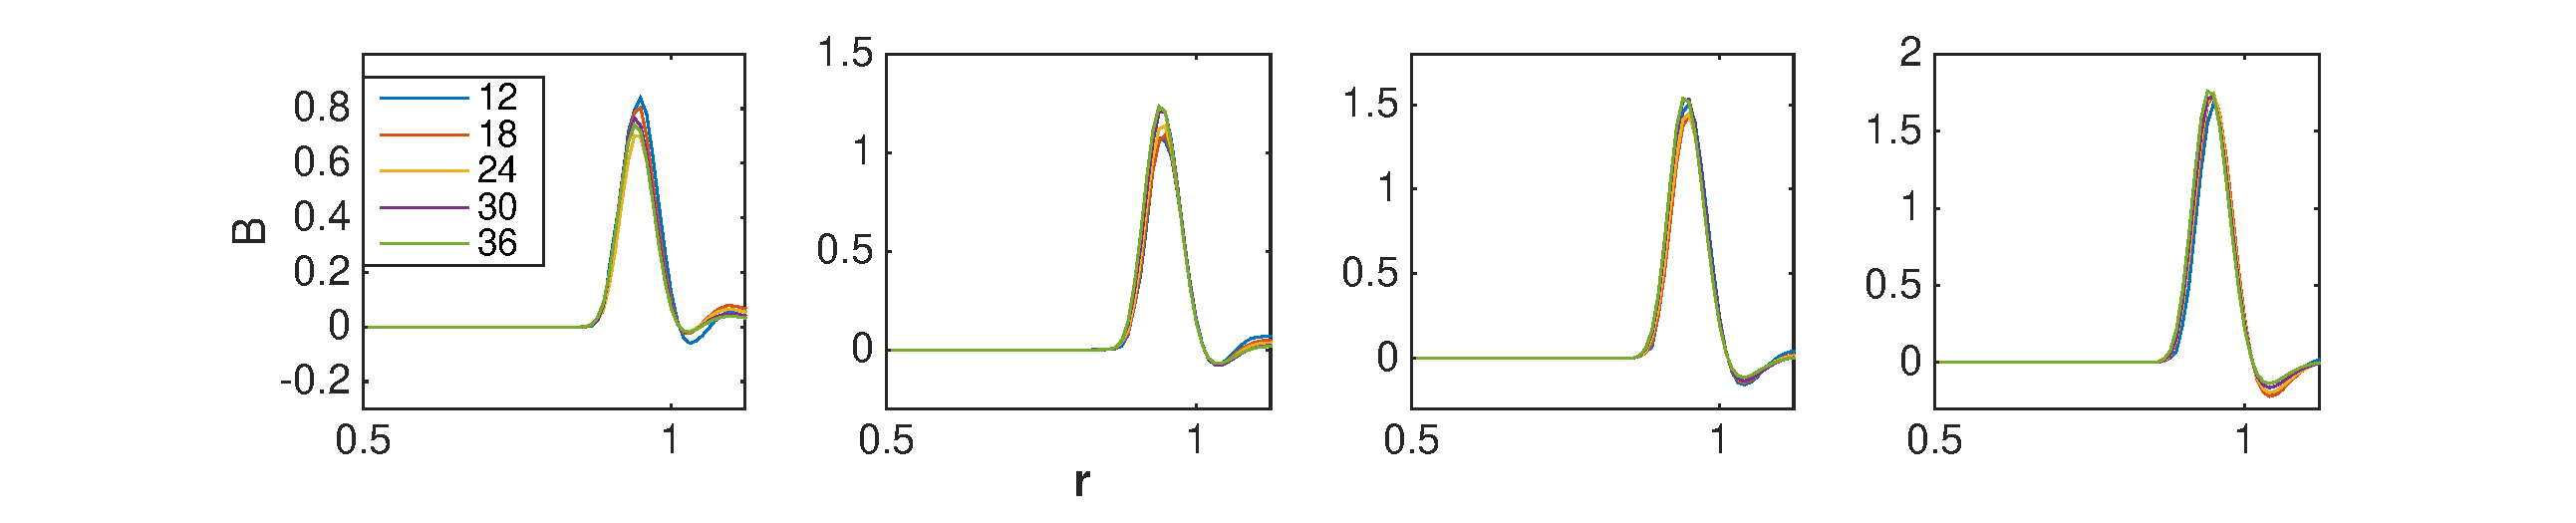
\includegraphics[width=1.0\linewidth]{del_u_sq-del_sq_u_overPesq.eps}
	\caption{\label{fig:kirk}
		(Top) Plot of ${\cal I} = \rho_0 \int \left[ T\nabla^2 u({\bf r}) - (\nabla u({\bf r}))^2\right] \Delta({\bf r}) \dd{\bf r}$ as a function of $\rm Pe$ at $\tau=\{20,30,40,50\}$, respectively from left to right. Fits are to ${\cal I} = a {\rm Pe} + b {\rm Pe}^2$. The maximum value of the ratio $b/a$ is $b/a \approx 5$ implying that the quadratic component is dominant for larger values of $Pe$. 
		(Bottom) Plot of $(1/{\rm Pe})^2 \left[T \nabla^2 u - (\nabla u)^2\right]$ as a function of the interparticle distance $r$ scaled by the particle diameter $\sigma=1$, for different values of ${\rm Pe}$. The four plots correspond to $\tau =\{20,30,40,50\}$, respectively from left to right.
	}
\end{figure*}


%{\color{red}Justify more precisely $\int\Omega({\bf r})\dd{\bf r}=0$, {\it i.e.} which symmetry is used}

To proceed further, we adapt Kirkwood's closure to approximate the three-body correlation $g_3$ in terms of some two-body correlations $g$. Specifically, we assume that $g_3({\bf r},{\bf r}') = c g_{\rm eq}({\bf r} - {\bf r}') g({\bf r}) g({\bf r}')$, where $c$ is a normalization factor that satisfies $g_3({\bf r} , {\bf r}') = c g_{\rm eq}({\bf r} - {\bf r}')g_{\rm eq}({\bf r})g_{\rm eq}({\bf r}')$ at equilibrium. Using the decomposition of $g$ in~\eqref{eq:g_dec}, we only keep terms up to order $\Delta $ in the isotropic correction. We first note that the terms involving a single factor of the anisotropic contribution $\Omega$ cancel to zero upon integration from symmetry considerations. Then, the only terms that survive are either quadratic in ${\rm Pe}.\Omega({\bf r})$ or linear in $\Delta({\bf r})$:
\begin{equation}\label{eq:Kirkwood}
	\begin{aligned}
		\frac{\gamma\dot w}{2} &= \rho_0\int \left[T\nabla^2 u({\bf r}) - (\nabla u({\bf r}))^2 \right] \Delta({\bf r}) \dd{\bf r} 
		\\
		&\quad - c \rho_0^2 \iint\dd{\bf r}\dd{\bf r}' \left[\nabla u({\bf r})\right] \cdot \left[\nabla u({\bf r}')\right] g_{\rm eq}({\bf r}-{\bf r}')
		\\
		&\qquad\times \big[ 2 \Delta({\bf r}) g_{\rm eq}({\bf r}') + {\rm Pe}^2 \Omega({\bf r}) \Omega({\bf r}') + {\cal O}(\Delta^2) \big] .
	\end{aligned}
\end{equation}
This is an integral equation relation between $\Delta$, $\delta$ and $\dot w$. Starting from the condition of energy balance~\eqref{eq:balance}, it provides an explicit constraint on how the density pair correlation $g$ is modified due to non-equilibrium driving. 


In order to probe the renormalization of the structure due to the non-equilibrium driving, we compute the isotropic component $\Delta$ of the nonequilibrium correction to density pair correlations $g-g_{\rm eq}$ from direct simulations of the microscopic dynamics~\eqref{eq:xEOM}. Then, we measure ${\cal I} = \rho_0 \int \left[ T\nabla^2 u({\bf r}) - (\nabla u({\bf r}))^2\right] \Delta({\bf r}) \dd{\bf r}$ as a function of $\rm Pe$ for various values of $\tau$. The choice of the specific combination ${\cal I}$ was motivated by the fact that in the limit of low density $\rho_0 \ll 1$ and weak tracer bath interactions, $h\ll 1$ Eq.~\ref{eq:Kirkwood} implies that ${\cal I}\propto \dot{w}\propto Pe^2$ to leading order in density and interaction strength.   

We observe that $\cal{I}$ scales linearly with $\rm Pe$ in the low $\rm Pe$ region, and scales quadratically in the high $\rm Pe$ region as reported in Fig.~\ref{fig:kirk}. Given that $\dot w = {\cal O}({\rm Pe}^2)$, the linear regime is not consistent with~\eqref{eq:Kirkwood}, thus suggesting a breakdown of the underlying closure relations, such as the Kirkwood approximation. In Fig.~\ref{fig:kirk}, we show that the integrand of $\cal I$ is well approximated by a scaling as ${\rm Pe}^2$ for ${\rm Pe}>30$. In short, while such a scaling is only confirmed numerically for large $\rm Pe$, our results suggest that~\eqref{eq:Kirkwood} is indeed useful to anticipate some constraints on the renormalization of density correlations due to nonequilibrium driving.


% ===============================================================================


\section{Biasing with energy flux renormalizes the interactions}

Finally, in order to investigate how energy fluxes affect the microscopic interactions in very general settings, we now consider biasing the dynamics in terms of the rate of potential energy stored in the tracer-bath interactions $\dd V/\dd t$, where $V$ is defined in Eq.~\ref{eq:Vdef}. This is based on modifying the particle trajectories by formally introducing an exponential weighting function $\ee^{ k . \varepsilon(t) }$ in the path probability of the microscopic dynamics~\eqref{eq:xEOM}, as defined within the framework of large deviations~\cite{Chetrite2013, Jack2010}. The variable $\varepsilon$ is extensive in time, and its rate $\varepsilon(t)/t$ is controlled by the bias amplitude $k$ at large time $t\to\infty$. Therefore, the biased ensemble enables one to probe some system configurations associated with different values of $\varepsilon(t)/t$, simply by monitoring the external parameter $k$.


For our purpose, we specifically choose $\varepsilon$ as
\begin{equation}\label{eq:eps}
	\varepsilon(t) = \frac{1}{\gamma} \int_0^t \left[ T\nabla_i^2 V + (\nabla_i V)\cdot({\bf F}_{{\rm d},i}+{\bf F}_i) \right] \dd s ,
\end{equation}
where ${\bf F}_i$ is the conservative force acting on particle $i$ and $i=0$ denotes the tracer particle. With this definition, $\varepsilon(t)/t \underset{t\to\infty}{\longrightarrow} \langle\dd V/\dd t\rangle_k$ according to Eqs.~(\ref{eq:V1}-\ref{eq:V2}), where $\langle\cdot\rangle_k$ denotes an average in the biased ensemble. In the unbiased case $k=0$, the energy flow vanishes $\langle\dd V/\dd t\rangle_0 = 0$. By tuning $k$ positive or negative, we generate trajectories that preferentially cause energy flow into or extract energy from the system, respectively for $\langle\dd V/\dd t\rangle_k>0$ and $\langle\dd V/\dd t\rangle_k<0$. Hence, sampling this ensemble of trajectories provides an indirect, if somewhat contrived, way to asses how energy flows can modify the properties of interacting many-body systems. We note that such trajectory biases have been used in other contexts for instance to explore dynamical heterogeneities in \textcolor{blue}{glassy systems~\cite{garrahan2007,Hedges2009,Pitard2011,Speck2012,Bodineau2012a,Limmer2014,Nemoto2017}, soliton solutions in high-dimensional chaotic chains~\cite{tailleur2007probing,laffargue2013} and the clustering of active self-propelled particles~\cite{Cagnetta2017,Whitelam2018,nemoto2018optimizing}.} 





As detailed in~\cite{Chetrite2013}, an auxiliary physical dynamics with the same averaged properties as in the biased ensemble can be constructed by solving the following eigenvalue equation 
\begin{equation}\label{eq:adjointbiased}
	\left[{\cal L}^\dagger + k \dot\varepsilon\right] g(k) = \lambda(k) g(k) ,
\end{equation}
where ${\cal L}^\dagger$ is the adjoint of the Fokker-Planck operator $\cal L$ ruling the time-evolution of the many-body probability distribution $p(\{{\bf r}_i\})$ as $\partial_t p = {\cal L} p$. The eigenvalue $\lambda(k)$ is the scaled cumulant generating function appropriate to the biasing function $\varepsilon$. The force field of the auxiliary dynamics $\tilde{\bf F}_i$ is defined in terms of the eigenfunction $g(k)$ as $\tilde {\bf F}_i = {\bf F}_i+ {\bf F}_{{\rm d},i} + \nabla_i \ln g(k)$. In practice, computing $\tilde {\bf F}_i$ is a highly non-trivial procedure for many-body systems, the explicit solutions obtained so far are only either perturbative or restricted to some mean-field dynamics~\cite{Nemoto2018a}.


An intuitive expression for the auxiliary force $\tilde{\bf F}_i$ can be obtained by solving~\eqref{eq:adjointbiased} perturbatively in terms of the bias $k$. Specifically, we expand $g(k)=g_0 + k g_1 + {\cal O}(k^2)$ and $\lambda(k)= \lambda_0 + k \lambda_1 + {\cal O}(k^2)$. Here, $g_0 = {\rm const.}$ is the uniform eigenvector of ${\cal L}^\dagger$ associated with $\lambda_0=0$. Substituting this expansion in~\eqref{eq:adjointbiased}, the leading order reads
\begin{equation}
		{\cal L}^\dagger g_1 = (\lambda_1 - \dot\varepsilon) g_0 .
\end{equation}
The operator ${\cal L}^\dagger$ can be readily written from the dynamics~\eqref{eq:xEOM} as ${\cal L}^\dagger = ({\bf F}_{{\rm d},i}+{\bf F}_i) \cdot \nabla_i + T \nabla^2_i$, and $\dot\varepsilon$ follows directly from the definition in~\eqref{eq:eps}. Besides, the leading eigenvalue is given by $\lambda_1 = \langle\dd V/\dd t\rangle_0 = 0$. We deduce that the solution for the leading non-trivial eigenvector is $g_1 = -(g_0/\gamma) V$. The force $\tilde{\bf F}_i$ of the auxiliary dynamics, which mimics the biased ensemble, then reads
\begin{equation}\label{eq:effectivedynamics}
	\begin{aligned}
		\tilde{\bf F}_i &= {\bf F}_i + {\bf F}_{{\rm d},i} +\nabla_i \ln \left[ g_0 + k g_1 + {\cal O}(k^2) \right]
		\\
		&= -k/\gamma \nabla_i V + {\bf F}_i+ {\bf F}_{{\rm d},i} + {\cal O}(k^2) .
	\end{aligned}
\end{equation}
As a result, the trajectories that consume energy from or release energy into the tracer-bath potential are associated with a physical dynamics where, at leading order, the tracer-bath interaction strength is simply renormalized by the bias amplitude $k$.
\begin{figure*}
	\centering
	\includegraphics[width=0.99\linewidth]{Fig4Full.pdf}
	\caption{\label{fig:energybias}
		(a) Plot of the tracer bath pair correlation function as a function of $k$. The driving force $Pe$ was turned off in these simulations. Estimates of the pair correlation function were obtained both from simulations of the biased ensemble \textcolor{blue}{using cloning algorithm} and from equilibrium simulations with Eq.~\ref{eq:effectivedynamics}. The two estimates are in good agreement. 
		(b) Plot of $\langle\dot{\epsilon}\rangle$ as a function of the biasing field $k$. The driving force $Pe$ was turned off in these simulations.  Estimates of $\langle\dot{\epsilon}\rangle$ were obtained both from simulations of the biased ensemble and from equilibrium simulations with Eq.~\ref{eq:effectivedynamics}. The two estimates are in good agreement. Together, these results show how energy biasing can modify the structure of the fluid. For values of $k>0$ when energy is pumped into the tracer bath interactions, the tracer and bath particles effectively repel each other more strongly in agreement with Eq.~\ref{eq:effectivedynamics}. Such enhanced repulsion can potentially favor phase separation of the tracer from the bath if there is a substantial concentration of tracers in the system.}
\end{figure*}



We tested the effectiveness of our theory by comparing averages generated from biased ensembles with those generated from equilibrium dynamics with Eq.~\ref{eq:effectivedynamics}. 
\textcolor{blue}{To generate the biased ensembles, we use the cloning algorithm~\cite{Giadina2006,tailleur2007probing,Hurtado2009,Nemoto2016,Ray2018,Klymko2018,Brewer2018}, where desired rare realizations (of simulations) are regularly selected and multiplied to efficiently sample the biased ensembles. (See Appendix A of \cite{Nemoto2016} for the detail of the implementation of the algorithm).}  
As opposed to simulations in the previous sections, the simulations here were performed with softer inter-particle interaction potentials, $V({\bf r})=\exp\left[-(1/(1-r^2/a^2))\right]$ where $a$ is the length scale at which the potential and all higher order derivatives vanish. In Fig.~\ref{fig:energybias}(a) we compare the tracer bath pair correlation function obtained from biased dynamics with those generated from equilibrium dynamics, chosen according to Eq.~\ref{eq:effectivedynamics}, for various values of the biasing field $k$. We find excellent agreement between the two radial distribution functions even for intermediate values of $|k|\sim 0.2$. In particular, in agreement with Eq.~\ref{eq:effectivedynamics}, the repulsion between the tracer and bath particles is increased when $k>0$ and decreased when $k<0$. 

In Fig.~\ref{fig:energybias}(b) we plot estimates of $\langle \dot{\epsilon} \rangle$ obtained both from biasing simulations and by applying Eq.~\ref{eq:effectivedynamics}, as a function of the biasing field $k$. Similar to Fig.~\ref{fig:energybias} (a), the two estimates of $\langle\dot{\epsilon}\rangle$ are in very good agreement even for intermediate values of $|k|\sim 0.2$. 
This agreement implies that the result of energy biasing can indeed be anticipated using our theory when in regimes where the biasing isn't strictly in a pertubative regime.




 Together, Fig.~\ref{fig:energybias} shows how energy flows\textendash obtained  by biasing using $k$ fields \textendash can be used to modulate the structure of the liquid in a controlled manner. They also provide intuition for the interplay between energy fluxes and structural reorganization in non-equilibrium systems. For instance, a positive value of $\langle \dot{\epsilon} \rangle$ reflects trajectories that are able to constantly pump energy into the tracer-bath interactions. Such trajectories might be typically observed in instances where the tracer is driven into the bath particle by external fields and energy is constantly pumped into the tracer bath interactions. This regime with $\langle \dot{\epsilon} \rangle >0 $ occurs where $k>0$. Eq.~\ref{eq:effectivedynamics} and Fig.~\ref{fig:energybias} predict that the effective repulsive interactions between the tracer and bath particles increases with $k>0$. In other words, trajectories that achieve  $\langle \dot{\epsilon} \rangle >0 $ and might be typical in instances where energy is actively pumped into the system by external driving forces, cause increased repulsions between the tracer and bath particles. If a substantial concentration of tracer particles is available, the effective increase in repulsive interactions between the tracer and bath particles can favor phase separation of the tracers from the bath. Such anticipated reorganization obtained by biasing energy flows is consistent with observed tradeoffs between energy consumption and organization in driven particle systems~\cite{delJunco2018}. Indeed, in these systems, phase separation occurs as amplitudes of the forces driving the particles, and hence the amount of energy being injected into the system, are increased~\cite{delJunco2018}. 


Alternatively, by choosing to bias a set of specific interactions with a vector of biasing variables $\{k\}$, it might be possible to promote spontaneous self assembly of various structures at the cost of energy consumption in such biased ensembles. Such a calculations can show how non-equilibrium flows can modify the information content and self-assembly dynamics of equilibrium landscapes~\cite{Murugan2015}.

% ===============================================================================


\section{Conclusion}

Developing techniques to characterize and control the behavior of far-from- equilibrium systems remains a central and outstanding problem in non-equilibrium thermodynamics. In this paper, we have shown that in certain limits, specifying simple scalar observables such as $\langle w \rangle$ or energy consumption rates allows us to constrain the transport and structural properties of our far-from-equilibrium system. It remains to be seen if similar results can be obtained in other more complex systems with anisotropic building blocks such as active liquid crystals or driven chiral objects~\cite{Joshi2017,vanZuiden2016,Nguyen2014b}. Such extensions will be pursued in future work.  


% ===============================================================================


\bibliographystyle{apsrev4-1}
\bibliography{Driven_ref.bib,DrivenDisks_v6.bib}

\end{document}

%
